\documentclass[12pt,a4paper]{beamer}
\usepackage[utf8]{inputenc}
\usepackage{amsmath}
\usepackage{amsfonts}
\usepackage{amssymb}
\usepackage{CJK}										% 支持中文
\usepackage{color}						% 给文字,表格和图形上色(68种)
\usepackage{xcolor}									% color包的扩展

%================================主题设置=============================%
\usetheme{Boadilla}									% PPT主题
\usefonttheme{serif} 
\useinnertheme{umbcboxes}


%================================具体设置=============================%
\setbeamercolor{umbcboxes}{bg=violet!12,fg=black}
\setbeamertemplate{navigation symbols}{}				% 取消引导
\hypersetup{colorlinks,citecolor = blue, linkcolor=blue}


	
%============================++++++++++++============================%
\author{hjy}
\title{presentation}
\institute{TongJi University}
\date{\today}	
%============================++++++++++++============================%	




\begin{document}
\begin{CJK*}{UTF8}{gkai}
%----------- titlepage ----------------------------------------------%
\begin{frame} 				
	\titlepage 
\end{frame}
	
%----------- outline ------------------------------------------------%
\begin{frame}
	\frametitle{目录}
	\tableofcontents
\end{frame}
  
%----------- slide	定义/pause的用法----------------------------------%
\begin{frame}
	\frametitle{幻灯片测试}
	\setlength{\fboxrule}{4pt} 
	\fcolorbox{red}{white}{我的第一张幻灯片。} 
	
	\pause
	\begin{definition}
		definition 1...
	\end{definition}
	
	\begin{proof}
  		We leave the proof as an exercise to our astute reader.
  		We also suggest that the reader generalize the proof to
  		non-Euclidean geometries.
	\end{proof}
\end{frame}
    
%----------- slide	公式/列表/公理------------------------------------%
\begin{frame}[label=sample]{A sample slide}
	A displayed formula:
	\[
		\int_{-\infty}^\infty e^{-x^2} \, dx = \sqrt{\pi}
	\]

	An itemized list:
	\begin{itemize}
  		\item itemized item 1
  		\item itemized item 2
	\end{itemize}

	\begin{theorem}
		In a right triangle, the square of hypotenuse equals
		the sum of squares of two other sides.
	\end{theorem}
	
	\begin{gather}
 		 u + iv = a \sin(x + iy) \\
  		u = a \sin x \cosh y, \\
  	 	\quad v = a \cos x \sinh y
	\end{gather}
\end{frame}

%----------- slide	链接---------------------------------------------%
\begin{frame}{Acknowledgment}
Fred Gornik, Power+Energy, Inc.\\
\href{http://powerandenergy.com}{http://powerandenergy.com}

\bigskip

If you click \hyperlink{sample}{here}, you will jump to the slide
labeled ``sample''.

Clicking \hyperlink{sample}{\beamerbutton{here}} will also
take you to the ``sample'' slide.

\bigskip
\beamerbutton{here} 
\beamergotobutton{here} 
\beamerskipbutton{here} 
\beamerreturnbutton{here} 

\end{frame}

%----------- slide	图片---------------------------------------------%
\begin{frame}{Hydrogen fuel cells: overview}
	\begin{center}
  		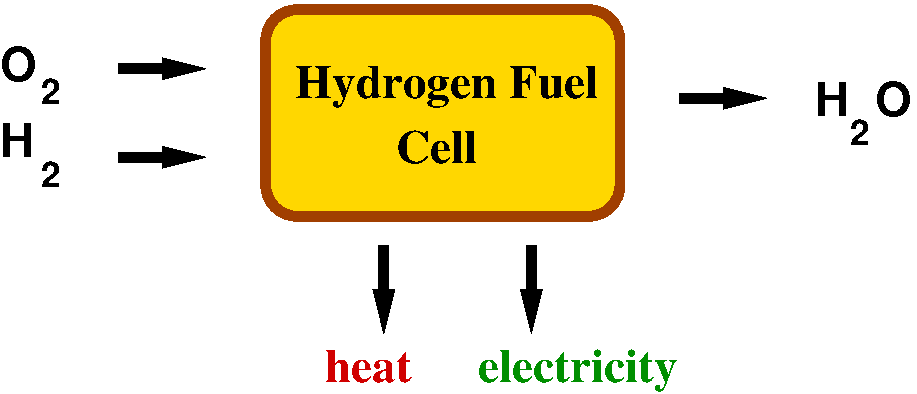
\includegraphics[height=3.0cm]{figs/schematic1.pdf}
	\end{center}
	\bigskip

	\pause

	\begin{center}
		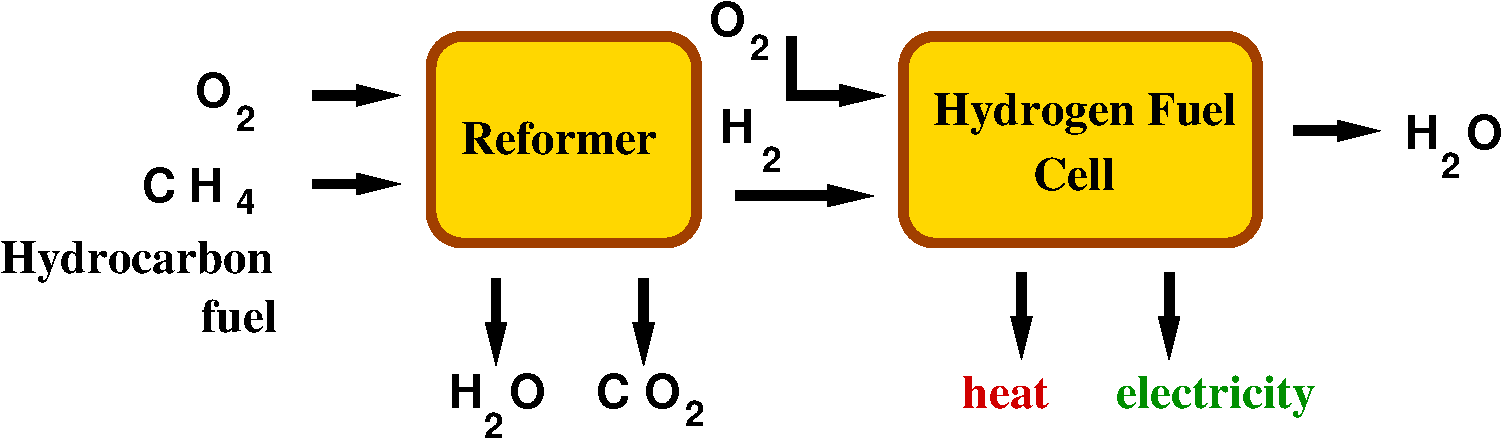
\includegraphics[height=3.0cm]{figs/schematic2.pdf}
	\end{center}
\end{frame}

%----------- slide	图片布局-----------------------------------------%
\begin{frame}{The Hydrogen-Palladium interface}

$\Gamma_0 = $ rate of hydrogen molecules impacting a surface

Representative value: $10^{19}$ hits/cm$^2$/sec

$\Gamma_0$ \emph{proportional} to pressure

\bigskip

\begin{columns}
  \begin{column}{.6\textwidth}
    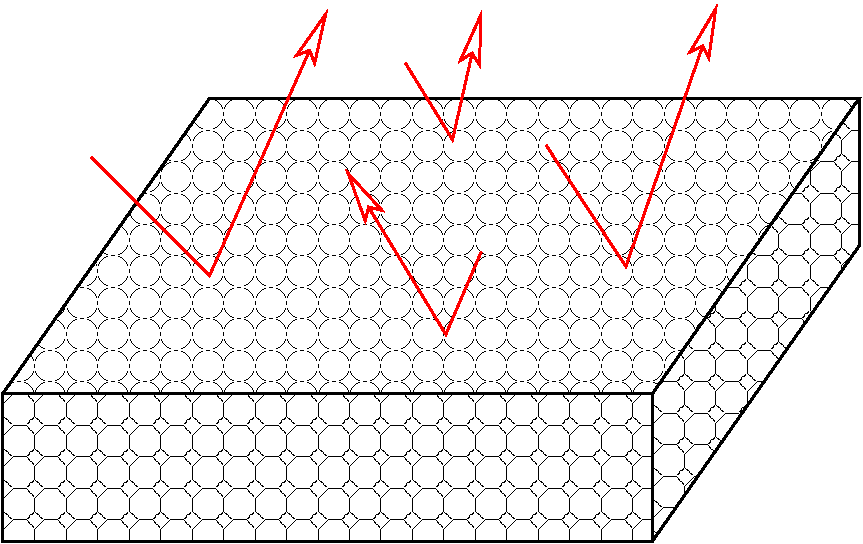
\includegraphics[width=0.8\textwidth]{figs/bounce.pdf}
    \smallskip

    Around $10^{14}$ surface sites/cm$^2$
  \end{column}
\pause
  \begin{column}{.3\textwidth}
    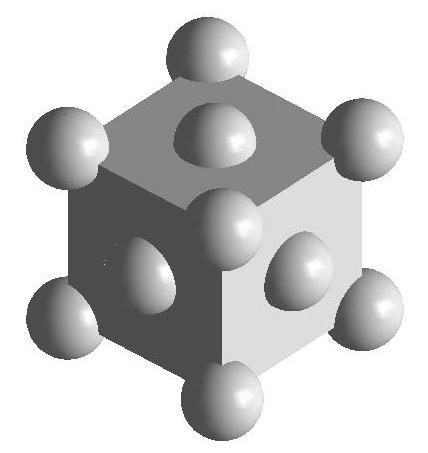
\includegraphics[width=\textwidth]{figs/fcc.jpg}
  \end{column}
\end{columns}
\end{frame}

%----------- slide	复杂公式-----------------------------------------%
\begin{frame}{Modeling the surface layer}

\structure{Equilibrium:}
\[
  \Gamma_0 S_0 (1-\alpha)^2 = k_d \alpha^2
  \quad \Rightarrow \quad
  \Bigl(\frac{1-\alpha}{\alpha}\Bigr)^2 = \frac{k_d}{\Gamma_0 S_0}
\]

Fraction of occupied surface sites on the surface $ = \alpha$, \quad
$0 \le \alpha \le 1$

\medskip

\begin{center}
  Solve for $P(x)$:\qquad
  \begin{onlinebox}{45mm} 
  	$\displaystyle P(x) = [ 1 + W(z)]^2$
  \end{onlinebox}
\end{center}

\medskip

\begin{displaybox}{90mm}
\[
  k_i \alpha (1-\beta) = k_o \beta (1-\alpha)
  \quad \Rightarrow \quad
  \frac{1-\alpha}{\alpha} = \frac{k_i}{k_o} \frac{1-\beta}{\beta}
\]

\[
  \text{Eliminate $\alpha$:} \qquad
  \frac{\beta}{1-\beta} = \frac{k_i}{k_o}
  \sqrt{\frac{\Gamma_0S_0}{k_d}} 
\]
\end{displaybox}
\end{frame}

%----------- slide	表格--------------------------------------------%
\begin{frame}{Numbers}


\renewcommand{\arraystretch}{1.7}
\begin{tabular}{lll}
  tube radius & $r$ & 0.3175 cm \\
  tube wall thickness & $\delta$ & 0.0003 cm \\
  flow rate & $F$ & 8330 cm$^3$/sec \\
  inlet pressure & $P(0)$ & 4.08 atm \\
  ambient pressure & $\rho$ & 1.36 atm \\
  temperature & $T$ & 673 Kelvin \\
  diffusivity & $\kappa$ & 6.96 10$^{-8}$ mol/(cm sec atm$^{1/2}$) \\
  gas constant & $R$ & cm$^3$ atm / (mol Kelvin)
\end{tabular}

\end{frame}

%----------- slide	表格--------------------------------------------%
\begin{frame}{Membrane on porous support}

\only<1>{
  \centerline{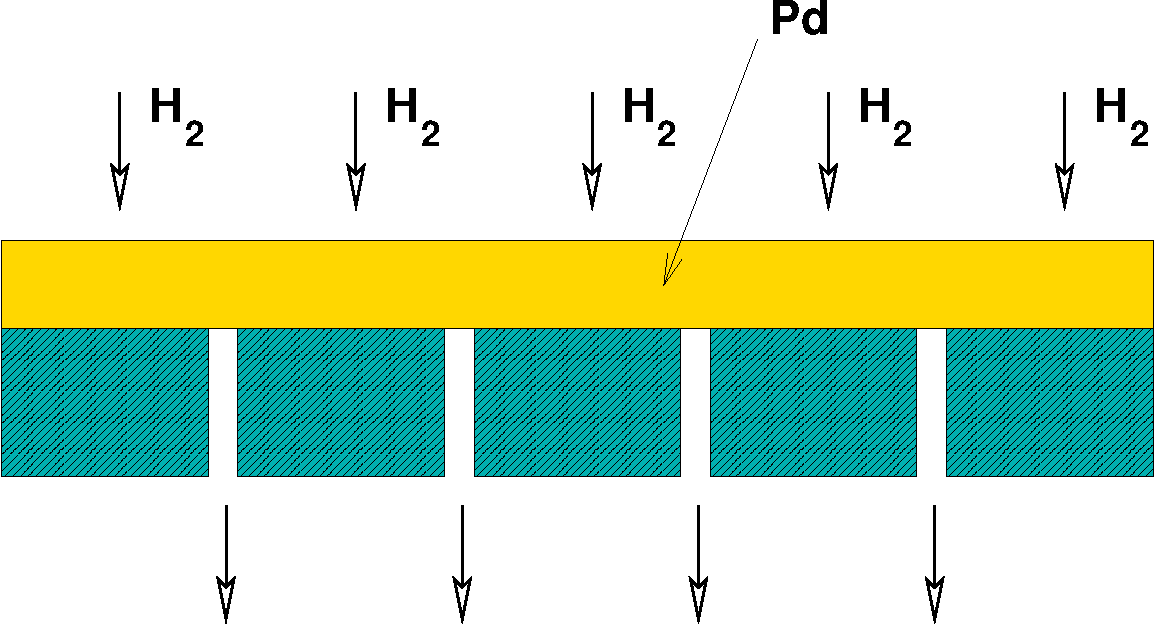
\includegraphics[height=4cm]{figs/bedsupport1.pdf}}
}

\onslide<2->{
  \centerline{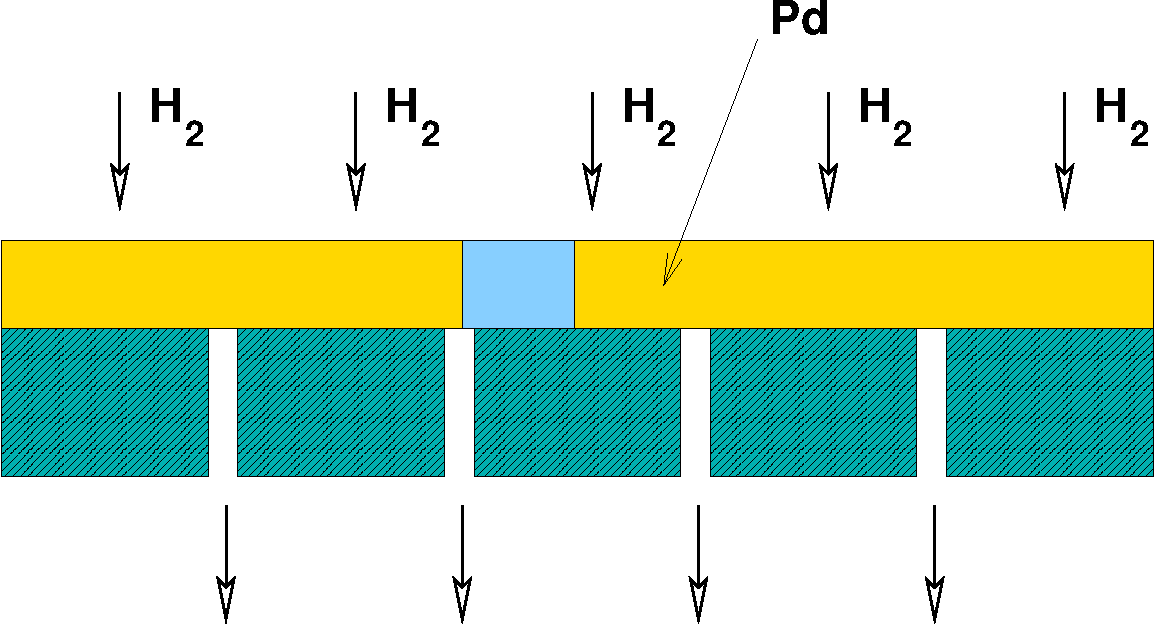
\includegraphics[height=4cm]{figs/bedsupport2.pdf}}
}

\onslide<3->{
\begin{columns}[T]
  \begin{column}{0.3\textwidth}
    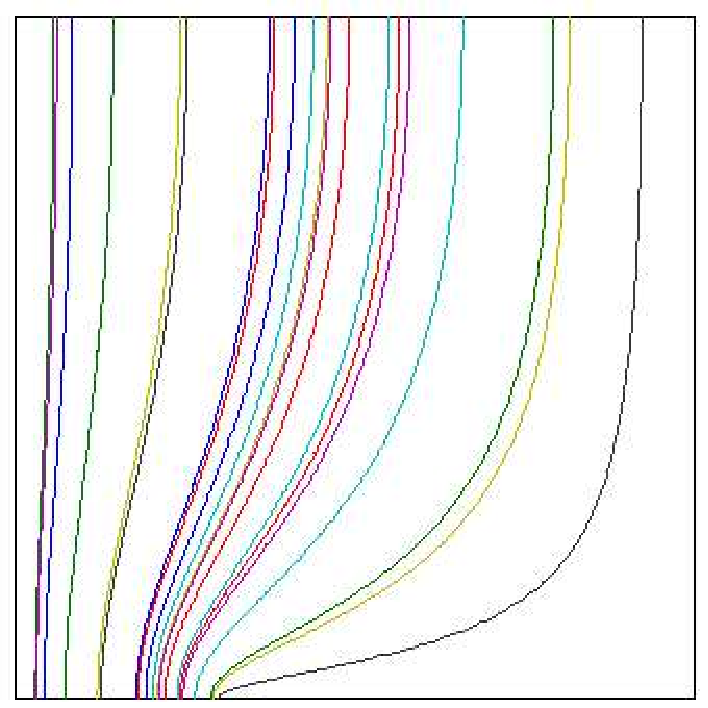
\includegraphics[height=26mm]{figs/cell-lines.pdf}
  \end{column}
  \begin{column}{0.3\textwidth}
    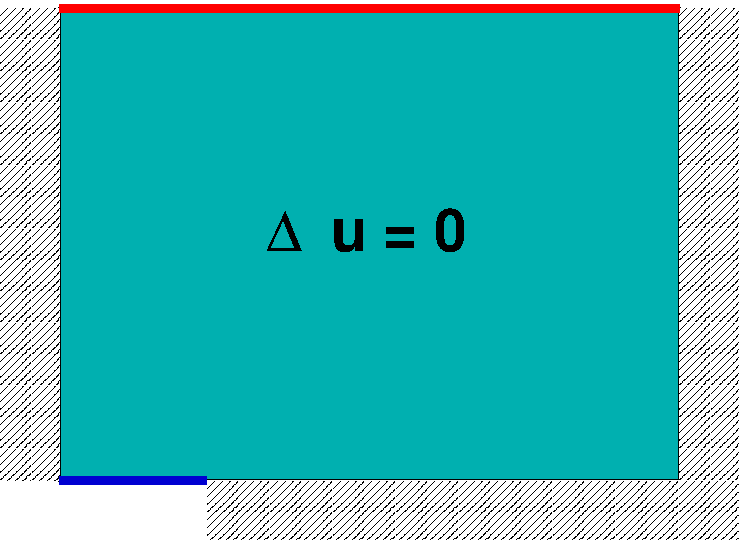
\includegraphics[height=29mm]{figs/bedsupport3.pdf}
  \end{column}
\end{columns}
}

\end{frame}

%----------- slide	表格--------------------------------------------%
\begin{frame}{Another title}
    Some text\\
    \uncover<2->{Uncover me on slide 2 (-)\\}
    \visible<3->{visible from slide 3 on (-)\\}
    \only<4->{only from slide 4 (-)\\} 
    \onslide<5->{on slide 5 and further (-)\\}
    \uncover<6>{Uncover me on slide 6 \\}
    \visible<7>{visible on 7\\}
    \only<8>{only on slide 8 \\} 
    \alt<8>{I am on slide 8\\}{I am not on slide 8\\}
    \onslide<9>{on slide 9\\}
\end{frame}



\end{CJK*}
\end{document}